\documentclass[t]{beamer} 
\usepackage{tikz}
\usepackage[all]{xy}
\usepackage{amsmath,amssymb}
\usepackage{hyperref}
\usepackage{graphicx}
\usepackage[noend]{algcompatible}
\usepackage{multirow}

\DeclareMathOperator*{\argmin}{arg\,min}
\DeclareMathOperator*{\Lik}{Lik}
\DeclareMathOperator*{\PoissonLoss}{PoissonLoss}
\DeclareMathOperator*{\Peaks}{Peaks}
\DeclareMathOperator*{\Segments}{Segments}
\DeclareMathOperator*{\argmax}{arg\,max}
\DeclareMathOperator*{\maximize}{maximize}
\DeclareMathOperator*{\minimize}{minimize}
\newcommand{\sign}{\operatorname{sign}}
\newcommand{\RR}{\mathbb R}
\newcommand{\ZZ}{\mathbb Z}
\newcommand{\NN}{\mathbb N}
\newcommand{\z}{$z = 2, 4, 3, 5, 1$} 

\newcommand{\algo}[1]{\textcolor{#1}{#1}}
\definecolor{PDPA}{HTML}{66C2A5}
\definecolor{CDPA}{HTML}{FC8D62}
\definecolor{GPDPA}{HTML}{4D4D4D}

% Set transparency of non-highlighted sections in the table of
% contents slide.
\setbeamertemplate{section in toc shaded}[default][100]
\AtBeginSection[]
{
  \setbeamercolor{section in toc}{fg=red} 
  \setbeamercolor{section in toc shaded}{fg=black} 
  \begin{frame}
    \tableofcontents[currentsection]
  \end{frame}
}

\begin{document}

\title{Efficient line search optimization of penalty functions in
  supervised changepoint detection}

\author{
  Toby Dylan Hocking --- toby.hocking@nau.edu\\ 
  joint work with my student Jadon Fowler\\
  Machine Learning Research Lab --- \url{http://ml.nau.edu}\\
  School of Informatics, Computing and Cyber Systems\\
  Northern Arizona University, USA\\
  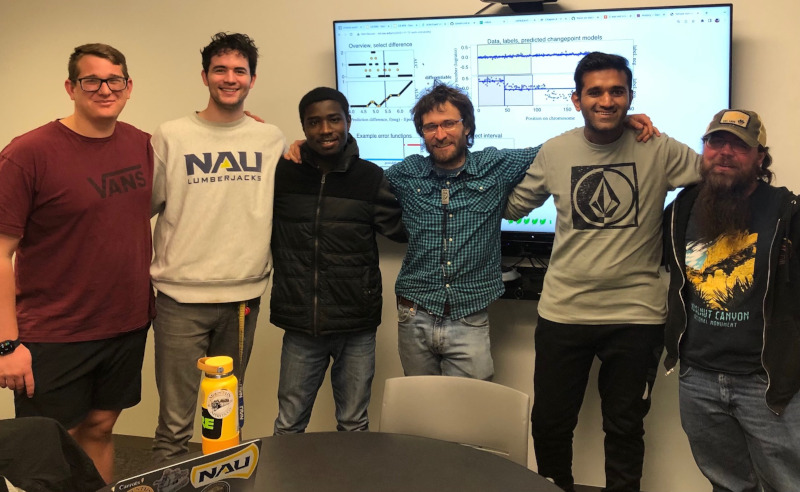
\includegraphics[height=4cm]{2023-02-02-group-meeting} \\
}

\date{}

\maketitle

\section{Problem Setting 1: ROC curves for evaluating supervised  binary classification algorithms}

\begin{frame}
  \frametitle{Problem: supervised binary classification}
  
  \begin{itemize}
  \item Given pairs of inputs $\mathbf x\in\mathbb R^p$ and outputs
    $y\in\{0,1\}$ can we learn a score 
    $f(\mathbf x)\in\mathbb R$, predict $y=1$ when $f(\mathbf x)>0$?
  \item Example: email, $\mathbf x =$bag of words, $y=$spam or not.
  \item Example: images. Jones {\it et al.} PNAS 2009.
    \parbox{2in}{\includegraphics[width=2in]{cellprofiler}}
    \parbox{1.9in}{Most algorithms (SVM, Logistic regression, etc) minimize a differentiable surrogate of zero-one loss = sum of:\\
      \textbf{False positives:} $f(\mathbf x)>0$ but $y=0$ (predict
      budding, but cell is not).\\
      \textbf{False negatives:} $f(\mathbf x)<0$ but $y=1$ (predict
      not budding but cell is).  }
  \end{itemize} 
\end{frame}

\begin{frame}
  \frametitle{Receiver Operating Characteristic (ROC) Curves}
  \begin{itemize}
  \item Classic evaluation method from the signal processing
    literature (Egan and Egan, 1975).
  \item For a given set of predicted scores, plot True Positive Rate
    vs False Positive Rate, each point on the ROC curve is a different
    threshold of the predicted scores.
  \item Best classifier has a point near upper left (TPR=1, FPR=0), with large
    Area Under the Curve (AUC).
  % \item Proposed idea: a new surrogate for AUC that is differentiable,
  %   so can be used for gradient descent learning.
  \end{itemize}
  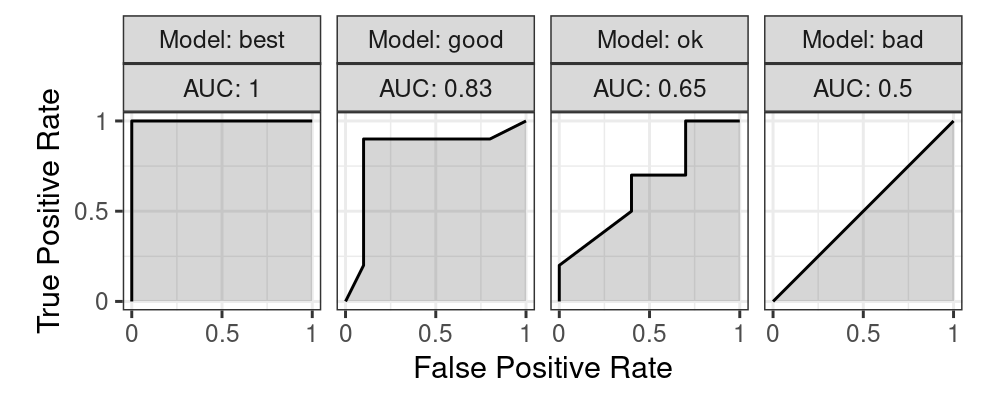
\includegraphics[width=\textwidth]{figure-more-than-one-binary}
\end{frame}

\begin{frame}
  \frametitle{Research question and new idea}
  Can we learn a binary classification function $f$ which directly
  optimizes the ROC curve?
  \begin{itemize}
  \item Most algorithms involve minimizing a differentiable surrogate
    of the zero-one loss, which is not the same.
  \item The Area Under the ROC Curve (AUC) is piecewise constant
    (gradient zero almost everywhere), so can not be used with
    gradient descent algorithms.
  \item We propose to encourage points to be in the upper left of ROC
    space, using a loss function which is a differentiable surrogate
    of the sum of min(FP,FN).
  \end{itemize}
  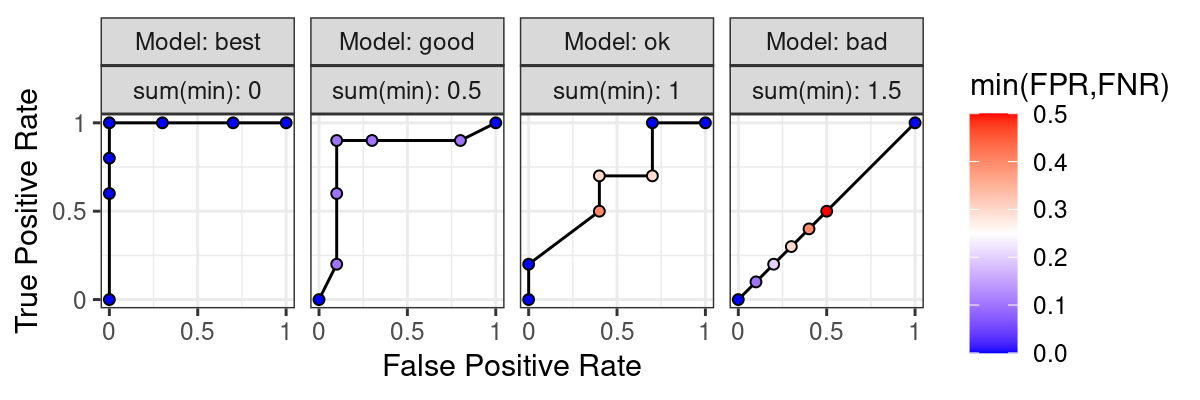
\includegraphics[width=\textwidth]{figure-more-than-one-binary-dots}
\end{frame}
 
\section{Problem setting 2: ROC curves for evaluating supervised changepoint algorithms}

\begin{frame}
  \frametitle{Problem: unsupervised changepoint detection}
  \begin{itemize}
  \item Data sequence $z_1,\dots,z_T$ at $T$ points over time/space.
  \item Ex: DNA copy number data for cancer diagnosis, $z_t\in\mathbb R$.
  \item The penalized changepoint problem (Maidstone \emph{et al.} 2017)
$$\argmin_{u_1,\dots,u_T\in\mathbb R} \sum_{t=1}^T (u_t - z_t)^2 + \lambda\sum_{t=2}^T I[u_{t-1} \neq u_t].$$
  \end{itemize}

  \parbox{0.6\textwidth}{
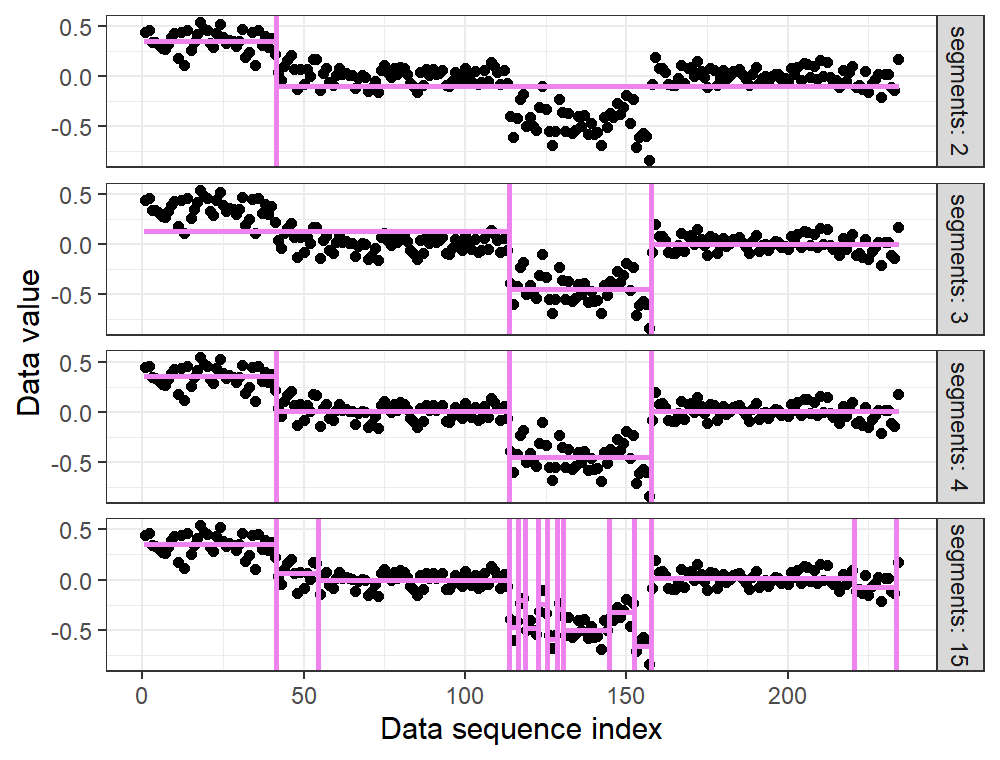
\includegraphics[width=0.6\textwidth]{figure-fn-not-monotonic-no-labels}
}
\parbox{0.3\textwidth}{
  Larger penalty $\lambda$ results in fewer changes/segments.

  \vskip 0.5in

  Smaller penalty $\lambda$ results in more changes/segments.
}

\end{frame}


\begin{frame}
  \frametitle{Problem: weakly supervised changepoint detection}
  \begin{itemize}
  \item First described by Hocking \emph{et al.} ICML 2013.
  \item We are given a data sequence $\mathbf z$ with labeled regions
    $L$.
  \end{itemize}

  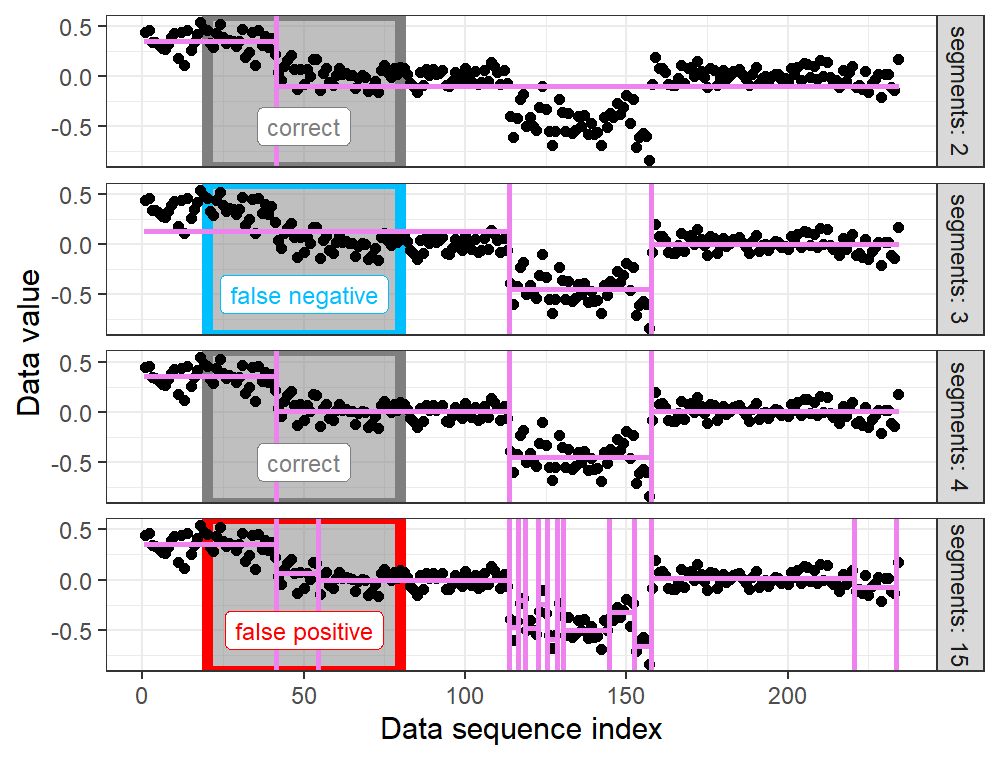
\includegraphics[width=0.56\textwidth]{figure-fn-not-monotonic}
  \only<2>{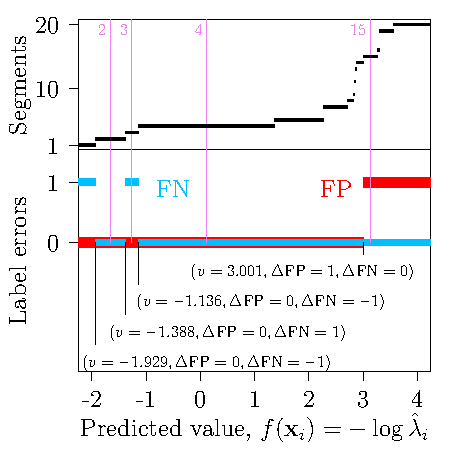
\includegraphics[width=0.42\textwidth]{figure-fn-not-monotonic-error-standAlone}}

  \only<2>{We compute features $\mathbf x=\phi(\mathbf z)\in\mathbf R^p$
    and want to learn a function $f(\mathbf x)=-\log\lambda\in\mathbf R$ that minimizes label error (sum of false positives and false negatives), or maximizes AUC.}

\end{frame}

\begin{frame}
  \frametitle{Comparing changepoint algorithms using ROC curves}
  Hocking TD, Srivastava A. Labeled Optimal
  Partitioning. Computational Statistics (2022).
  
  \includegraphics[width=0.8\textwidth]{figure-LOPART-roc}

  LOPART algorithm (R package LOPART) has consistently larger
  test AUC than previous algorithms.
\end{frame}

\section{Proposed complete line search algorithm for surrogate loss: Area Under Min\{FP,FN\} (AUM)} 

\begin{frame}
  \frametitle{Large AUC $\approx$ small Area Under Min(FP,FN) (AUM)} 
  
  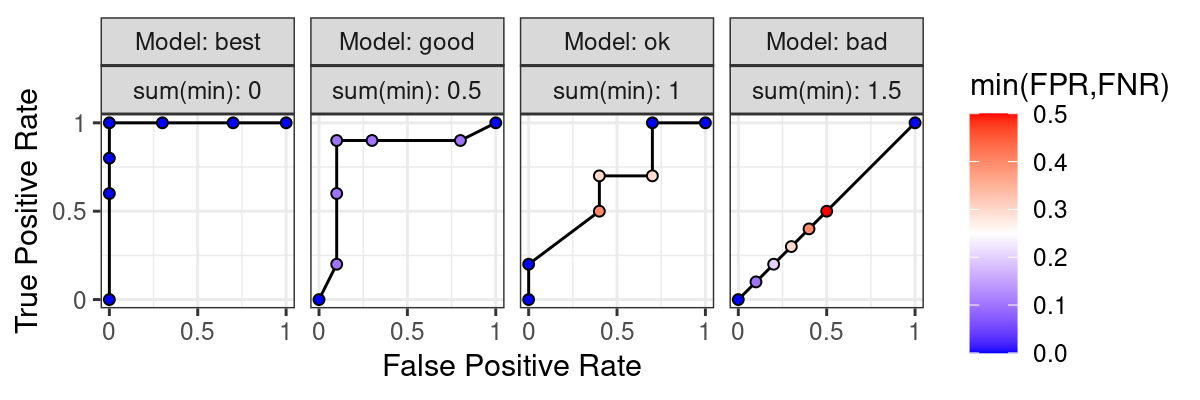
\includegraphics[height=1.3in]{figure-more-than-one-binary-dots}

  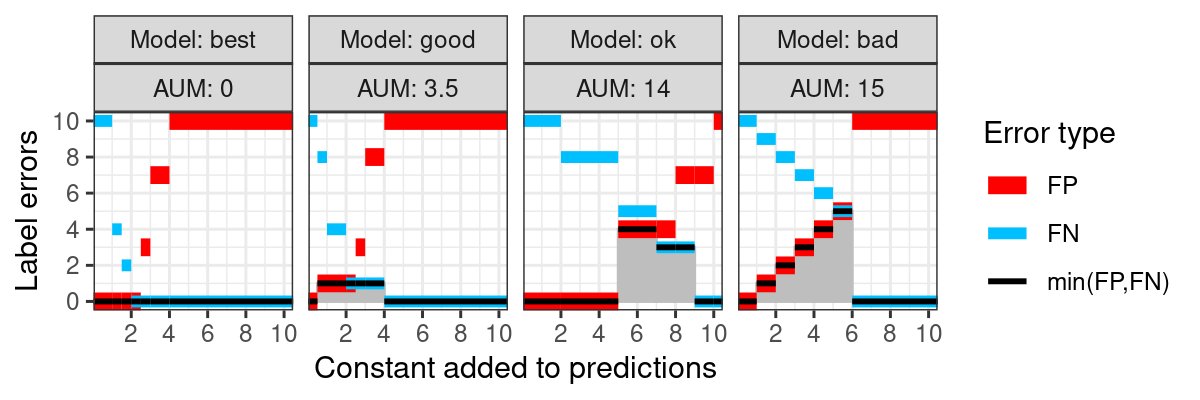
\includegraphics[height=1.3in]{figure-more-than-one-binary-aum}

  Barr, Hocking, Morton, Thatcher, Shaw, \emph{TransAI} (2022).

  Hocking, Hillman, \emph{Journal of Machine Learning Research} (2023).

  Proposal: track how thresholds in error plot change with step size.
  
\end{frame}

\begin{frame}
  \frametitle{Proposed line search algorithm uses AUC/AUM structure}

  Theorem: when learning a linear model, 
  \begin{itemize}
  \item AUC is piecewise constant, and
  \item AUM is piecewise linear,
  \end{itemize}
  as a function of step size in gradient descent.
  
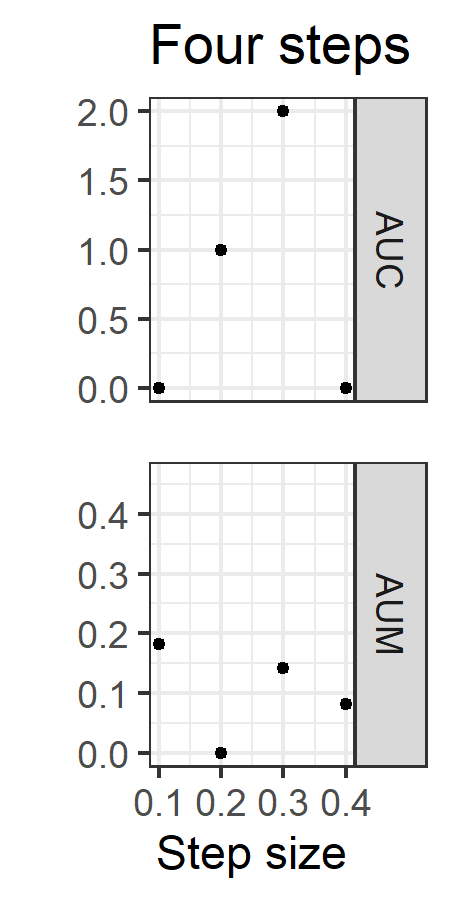
\includegraphics[height=5cm]{figure-line-search-example-some}
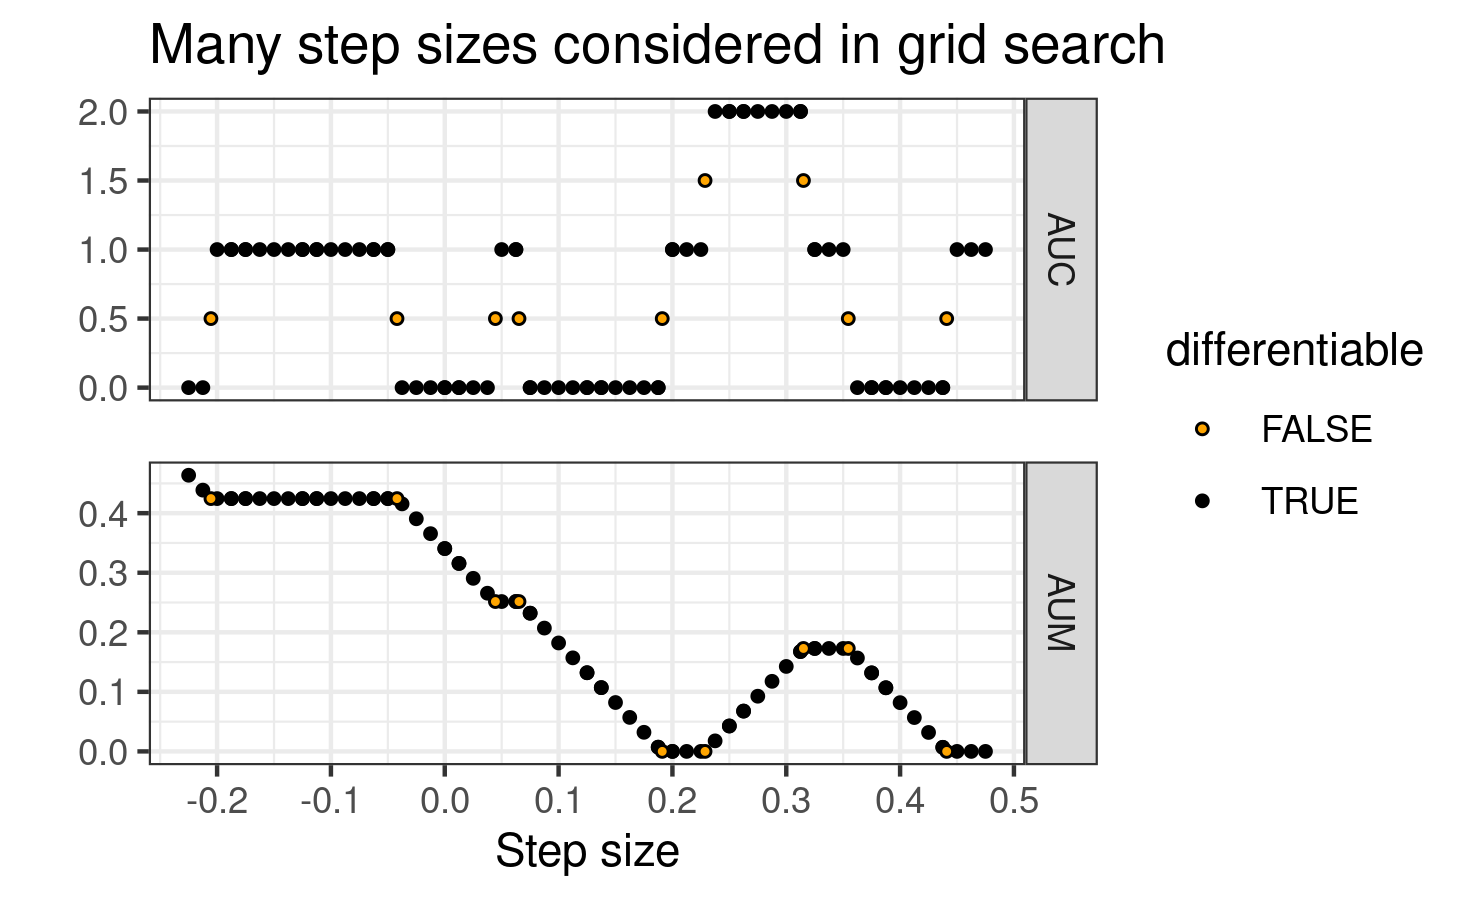
\includegraphics[height=5cm]{figure-line-search-example-grid}
 
Proposed line search algorithm computes updates when there are
possible changes in slope of AUM / values of AUC (orange dots).

\end{frame}


\begin{frame}
  \frametitle{AUM/AUC line search, iteration 1}
  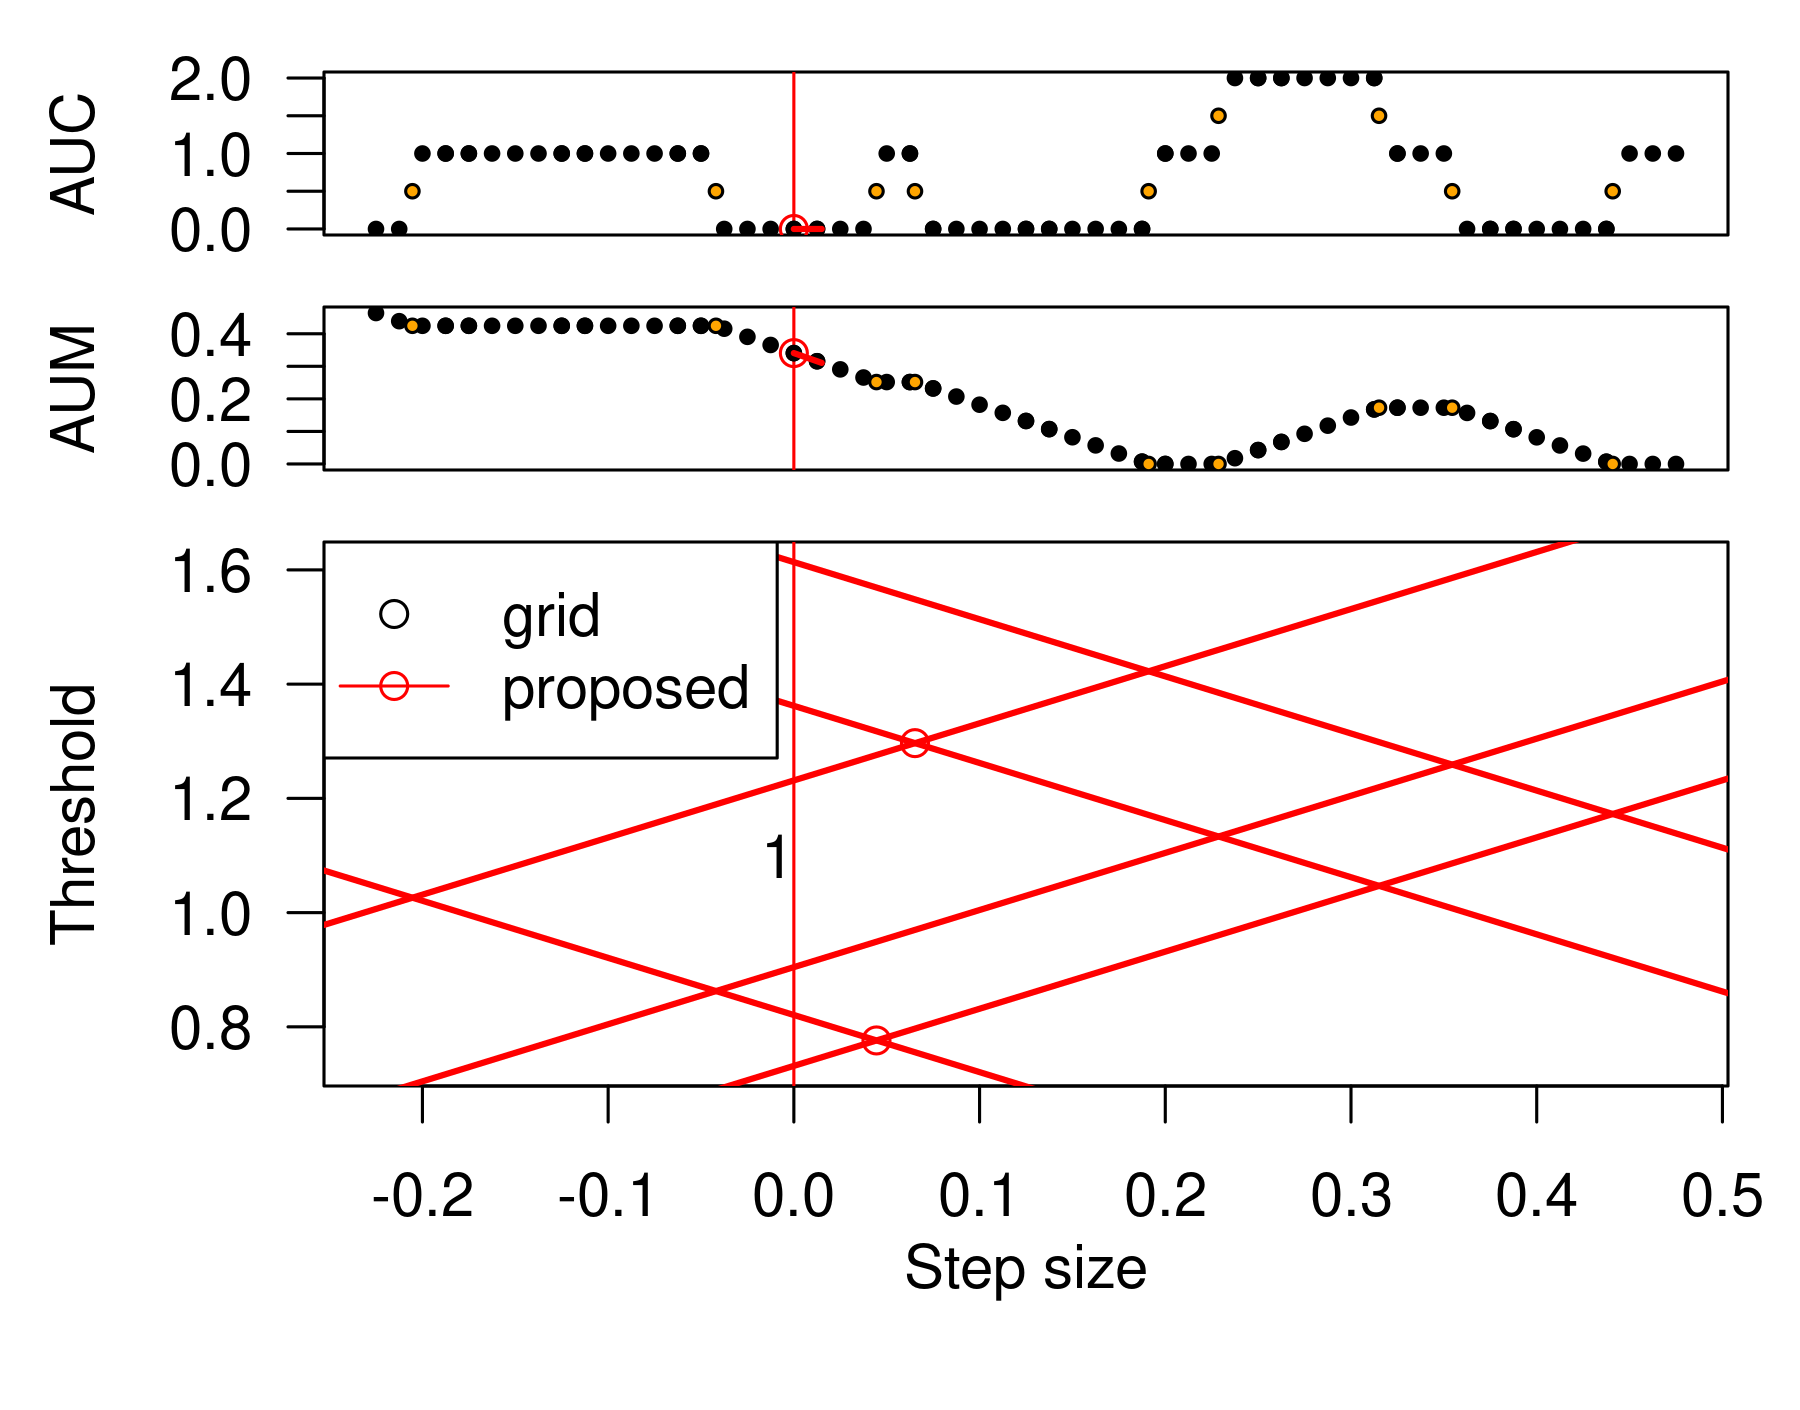
\includegraphics[width=\textwidth]{figure-line-search-example-1}
\end{frame}


\begin{frame}
  \frametitle{AUM/AUC line search, iteration 2}
  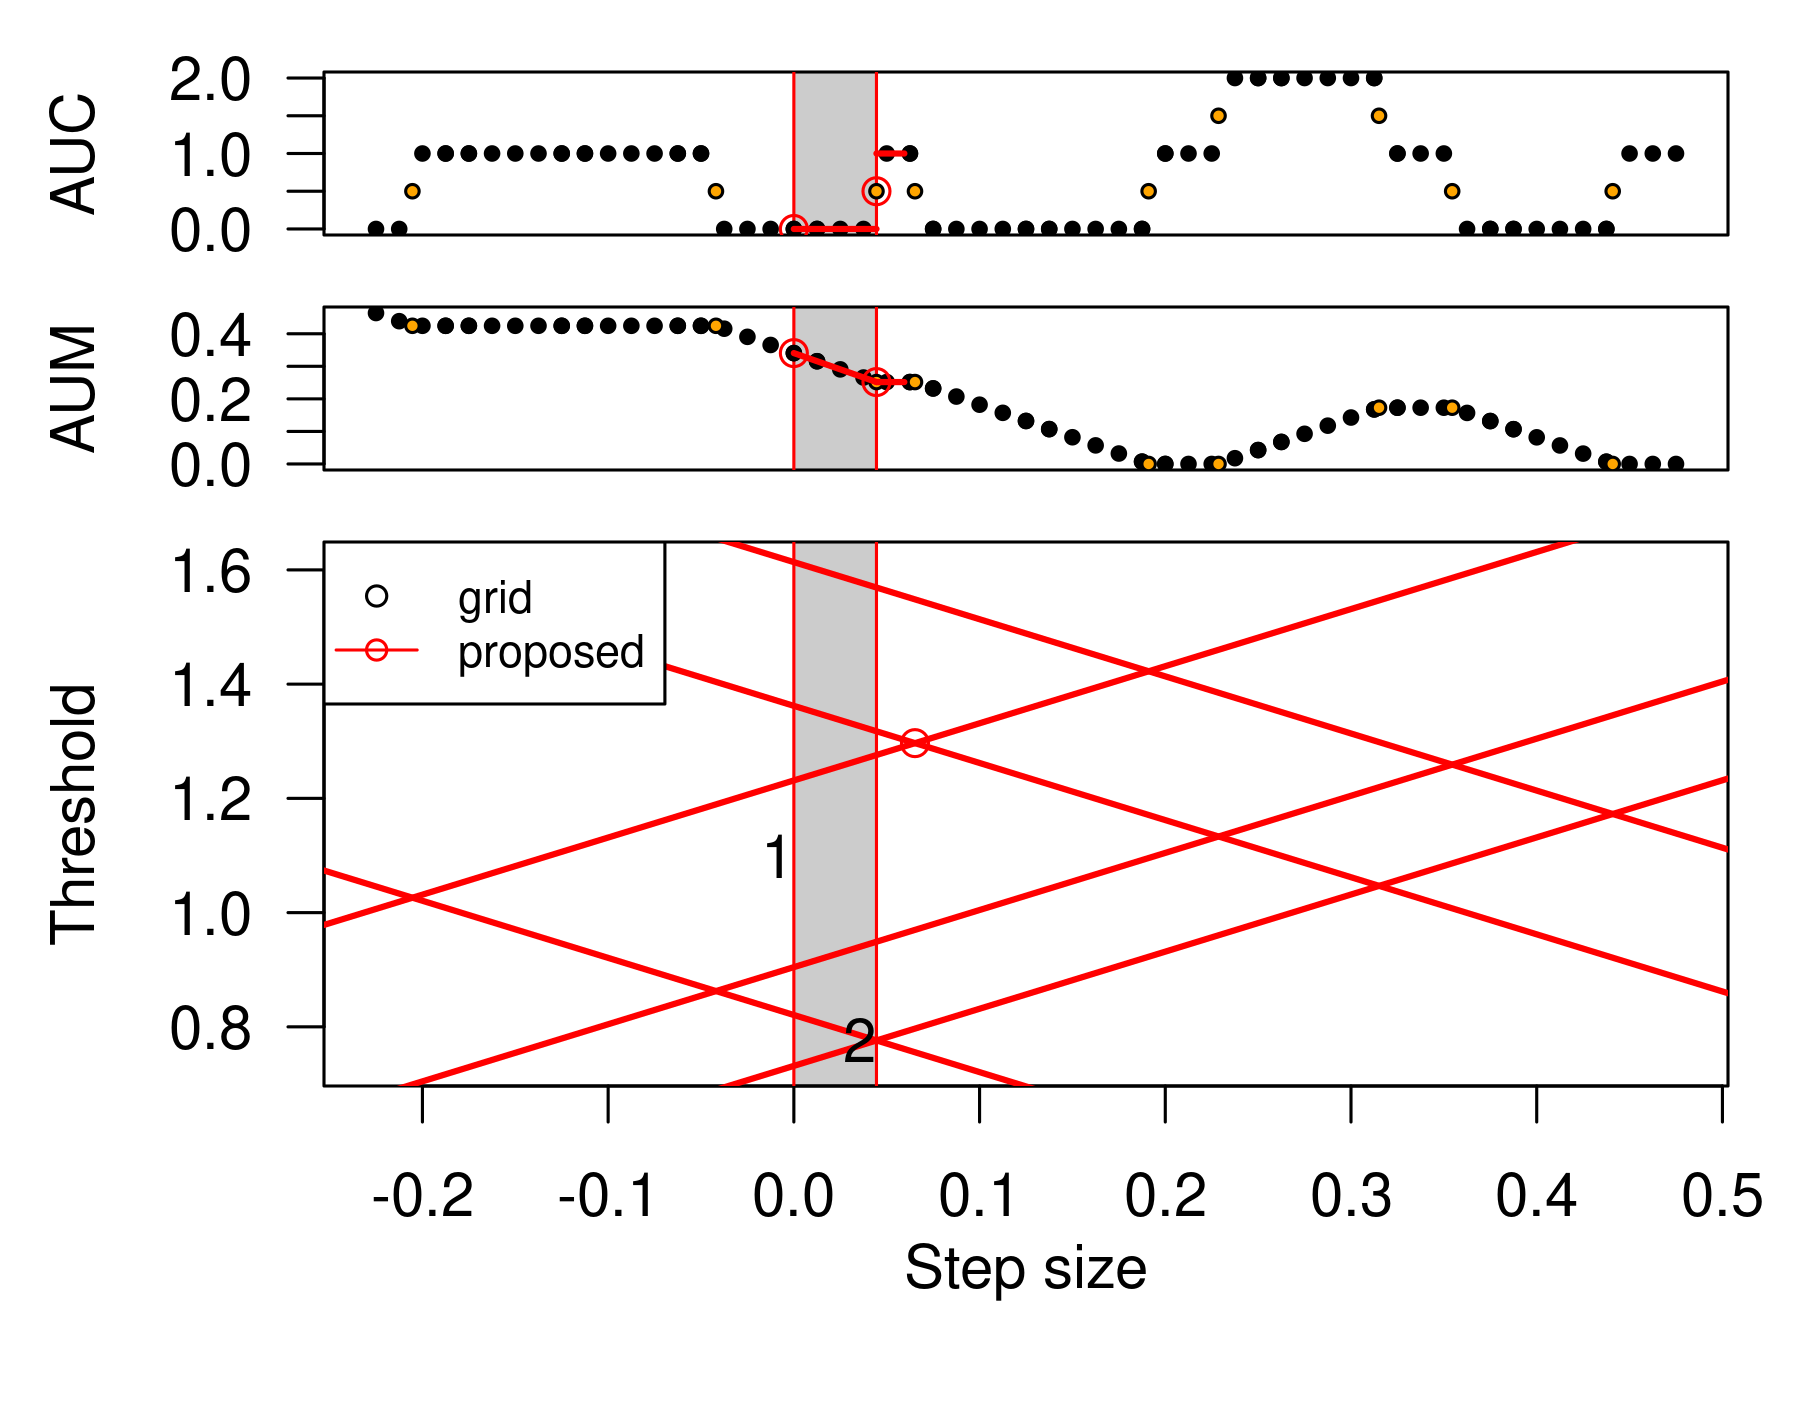
\includegraphics[width=\textwidth]{figure-line-search-example-2}
\end{frame}


\begin{frame}
  \frametitle{AUM/AUC line search, iteration 3}
  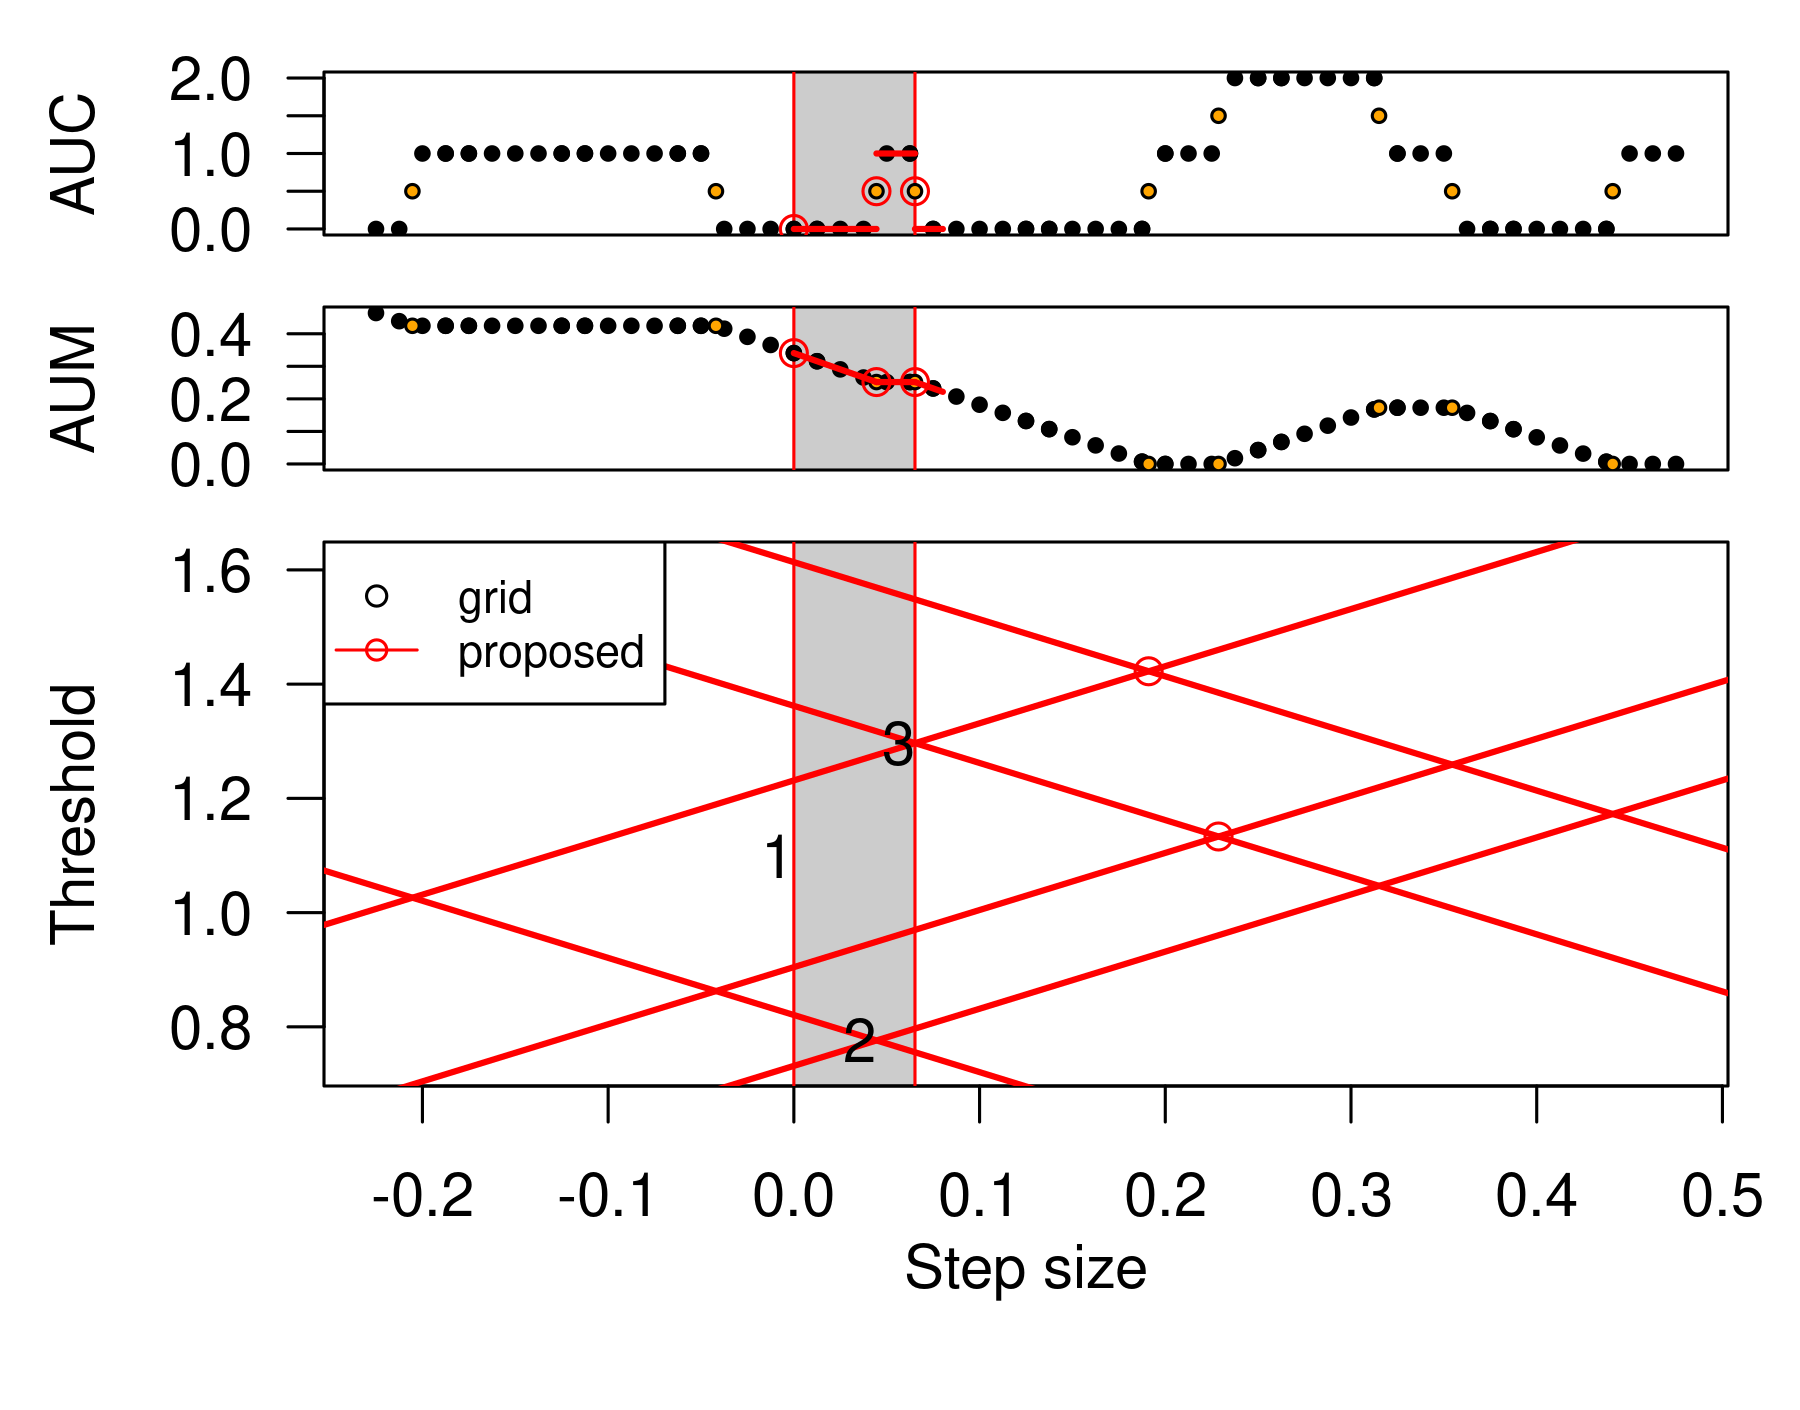
\includegraphics[width=\textwidth]{figure-line-search-example-3}
\end{frame}


\begin{frame}
  \frametitle{AUM/AUC line search, iteration 4}
  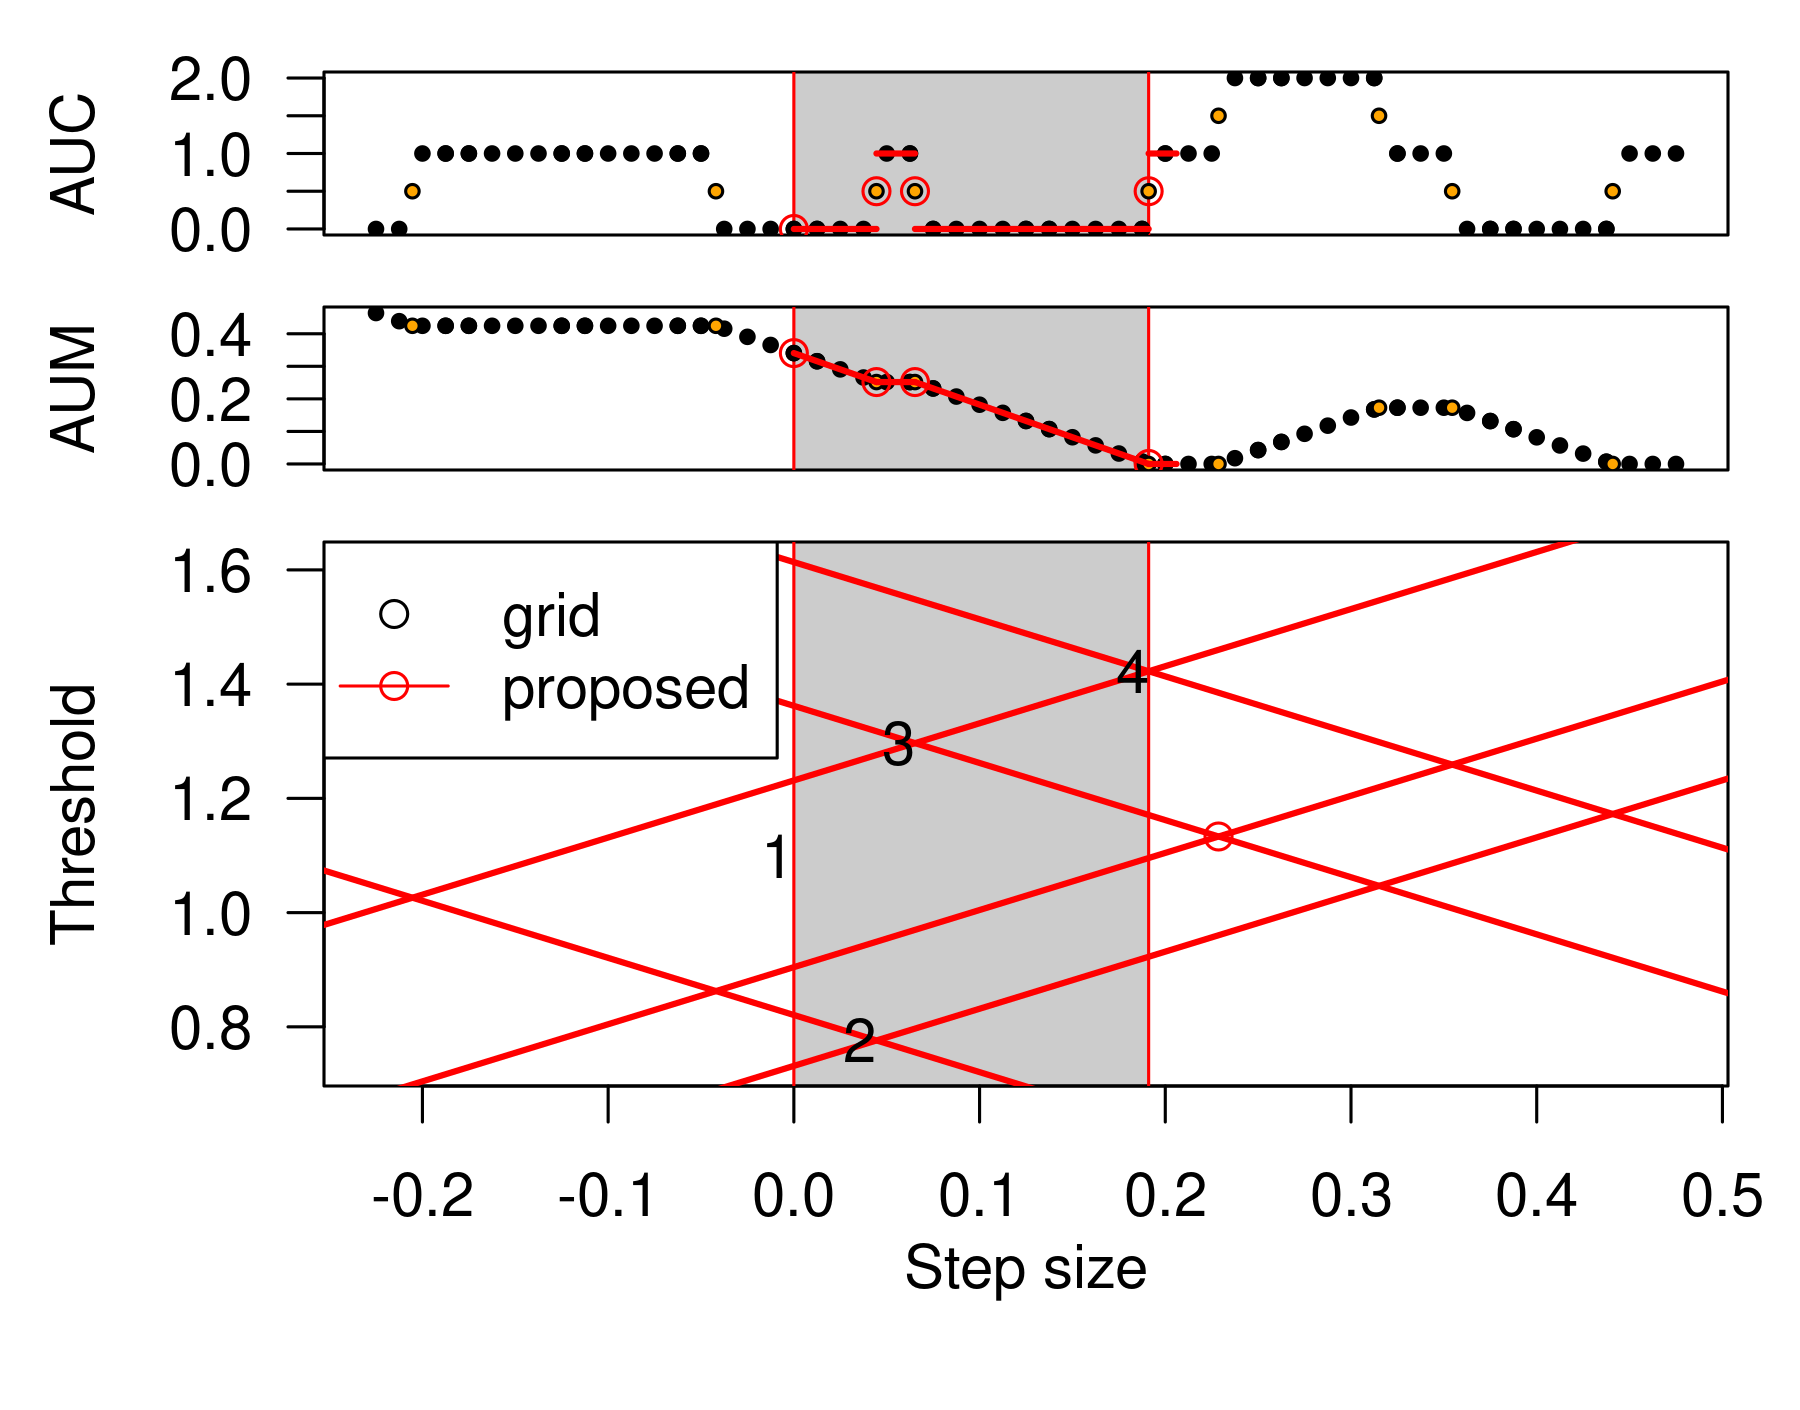
\includegraphics[width=\textwidth]{figure-line-search-example-4}
\end{frame}


\begin{frame}
  \frametitle{AUM/AUC line search, iteration 5}
  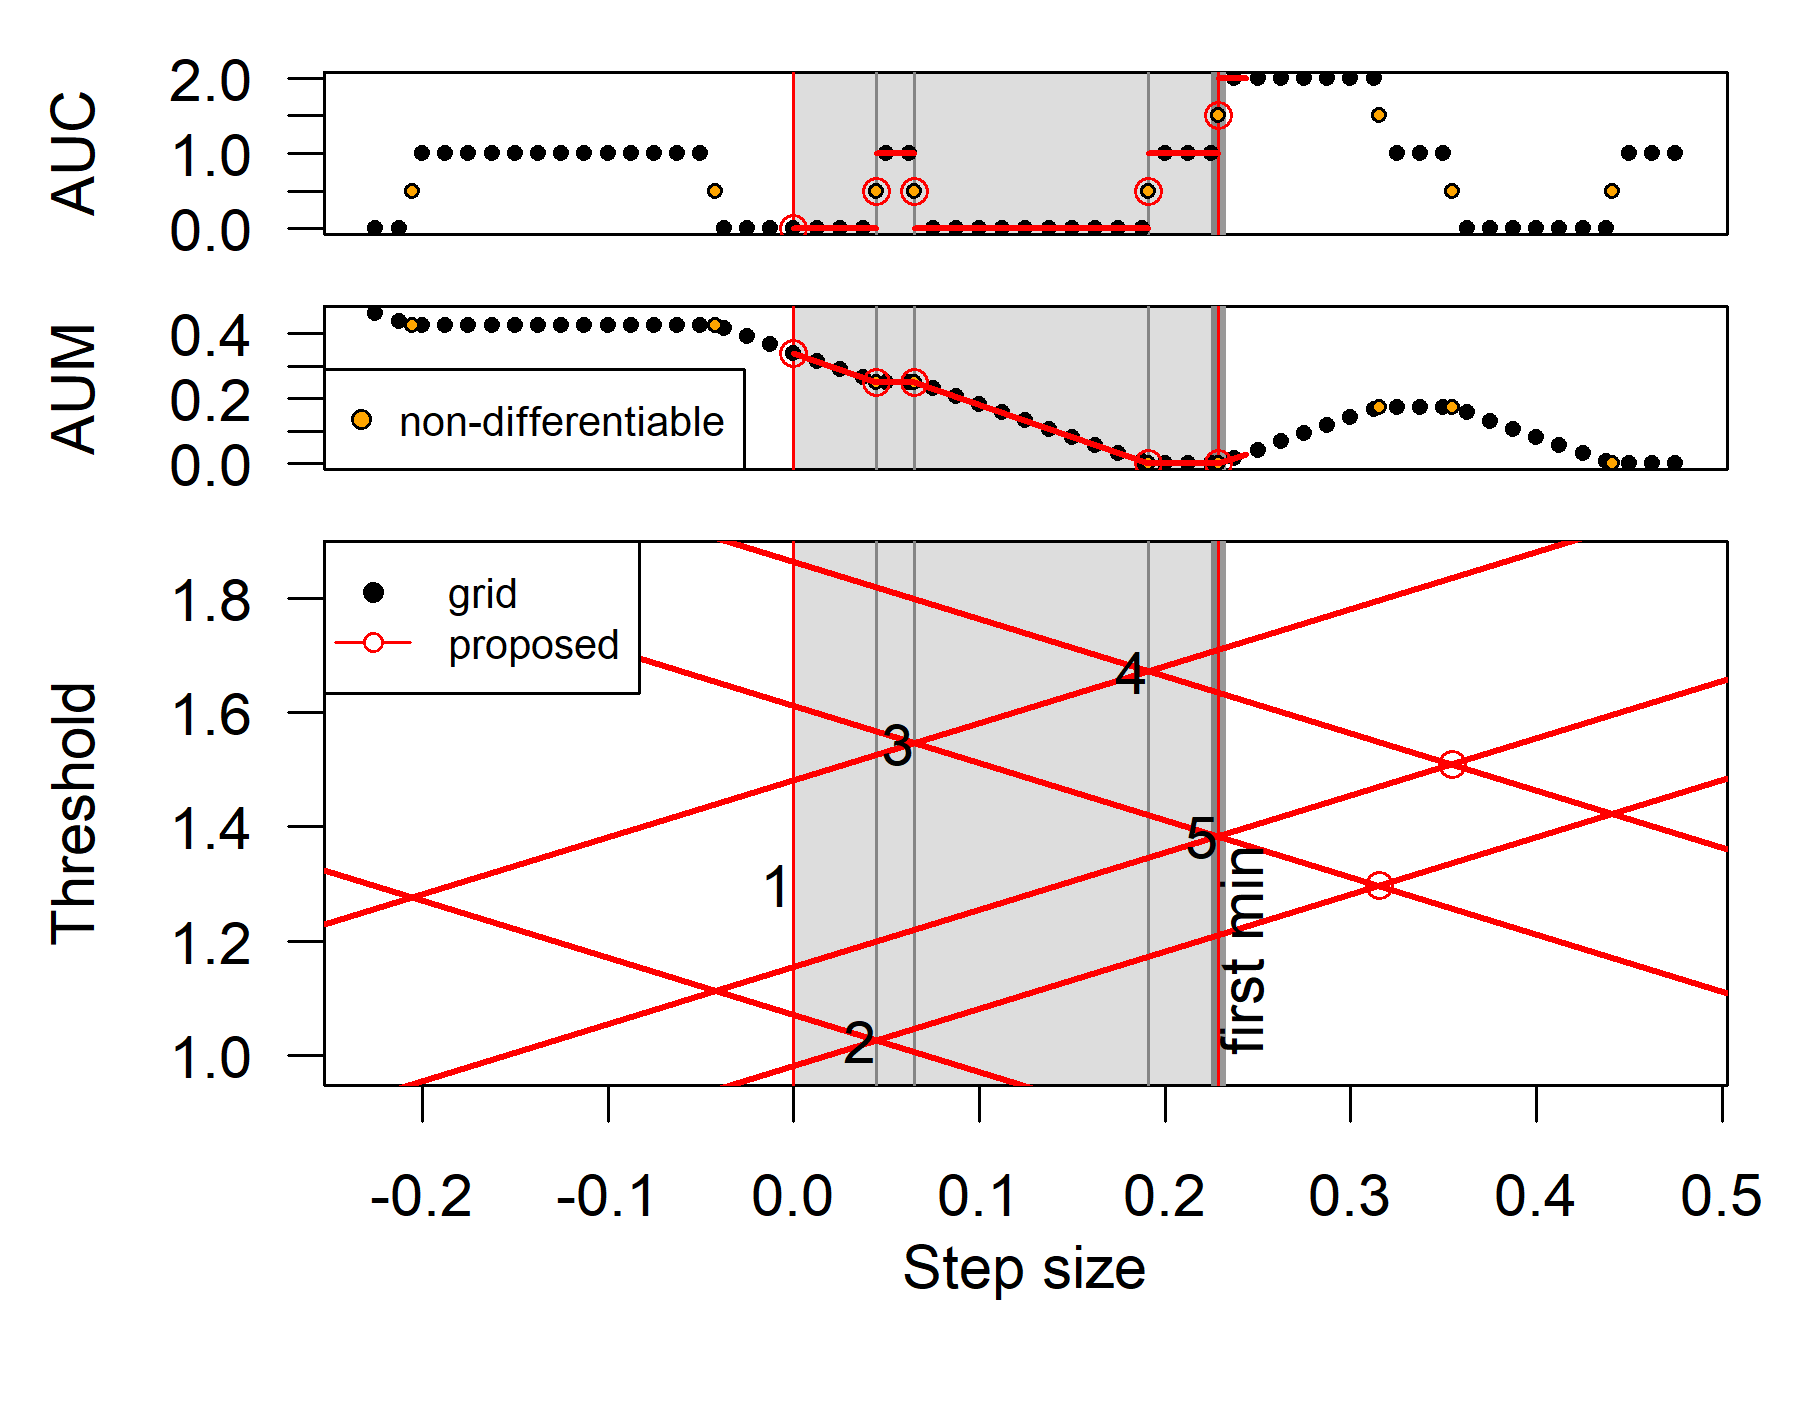
\includegraphics[width=\textwidth]{figure-line-search-example-5}
\end{frame}


\begin{frame}
  \frametitle{AUM/AUC line search, iteration 6}
  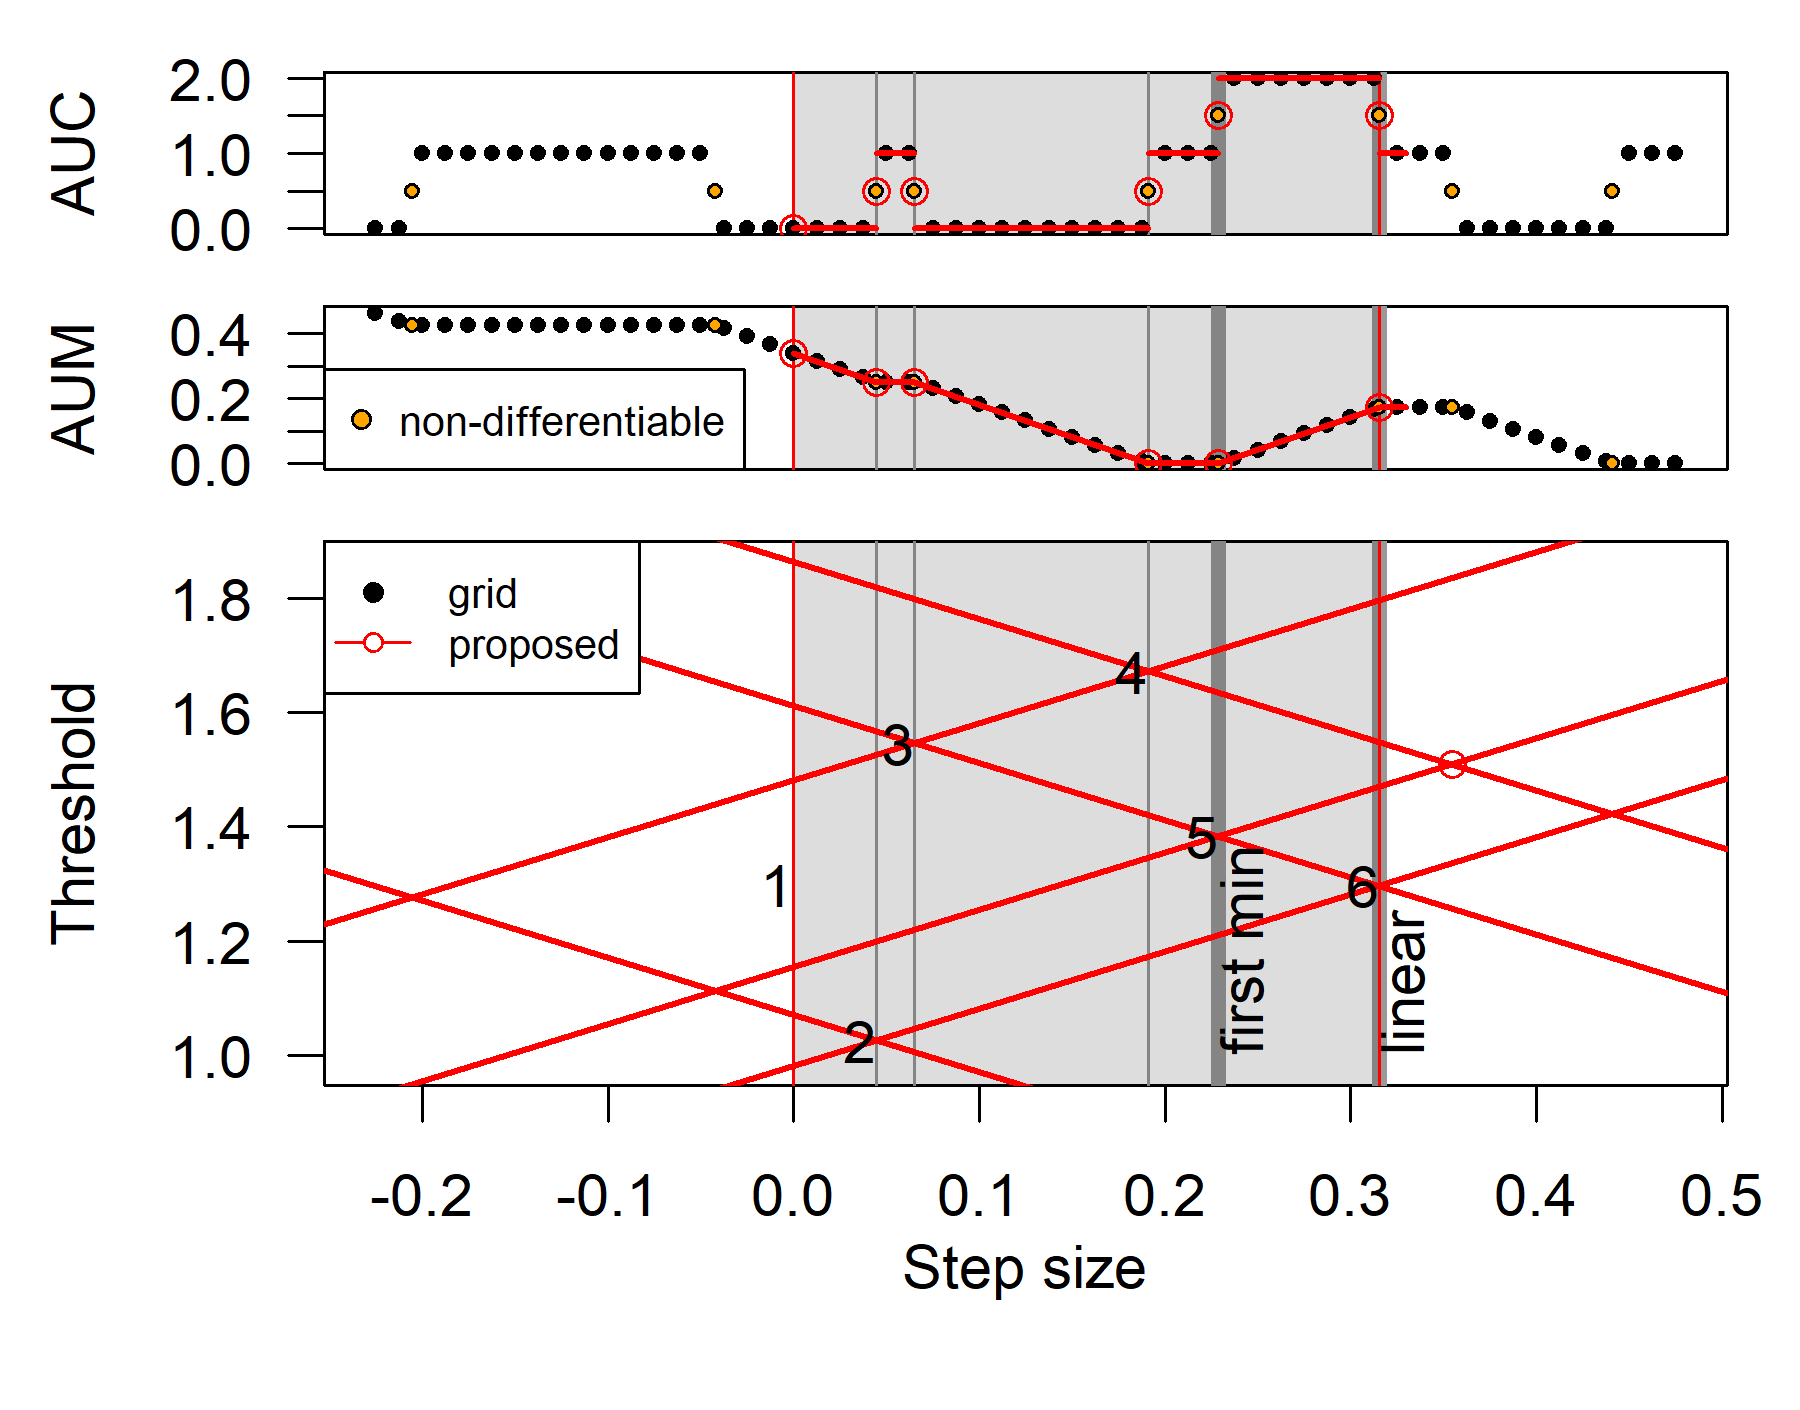
\includegraphics[width=\textwidth]{figure-line-search-example-6}
\end{frame}


\begin{frame}
  \frametitle{AUM/AUC line search, iteration 7}
  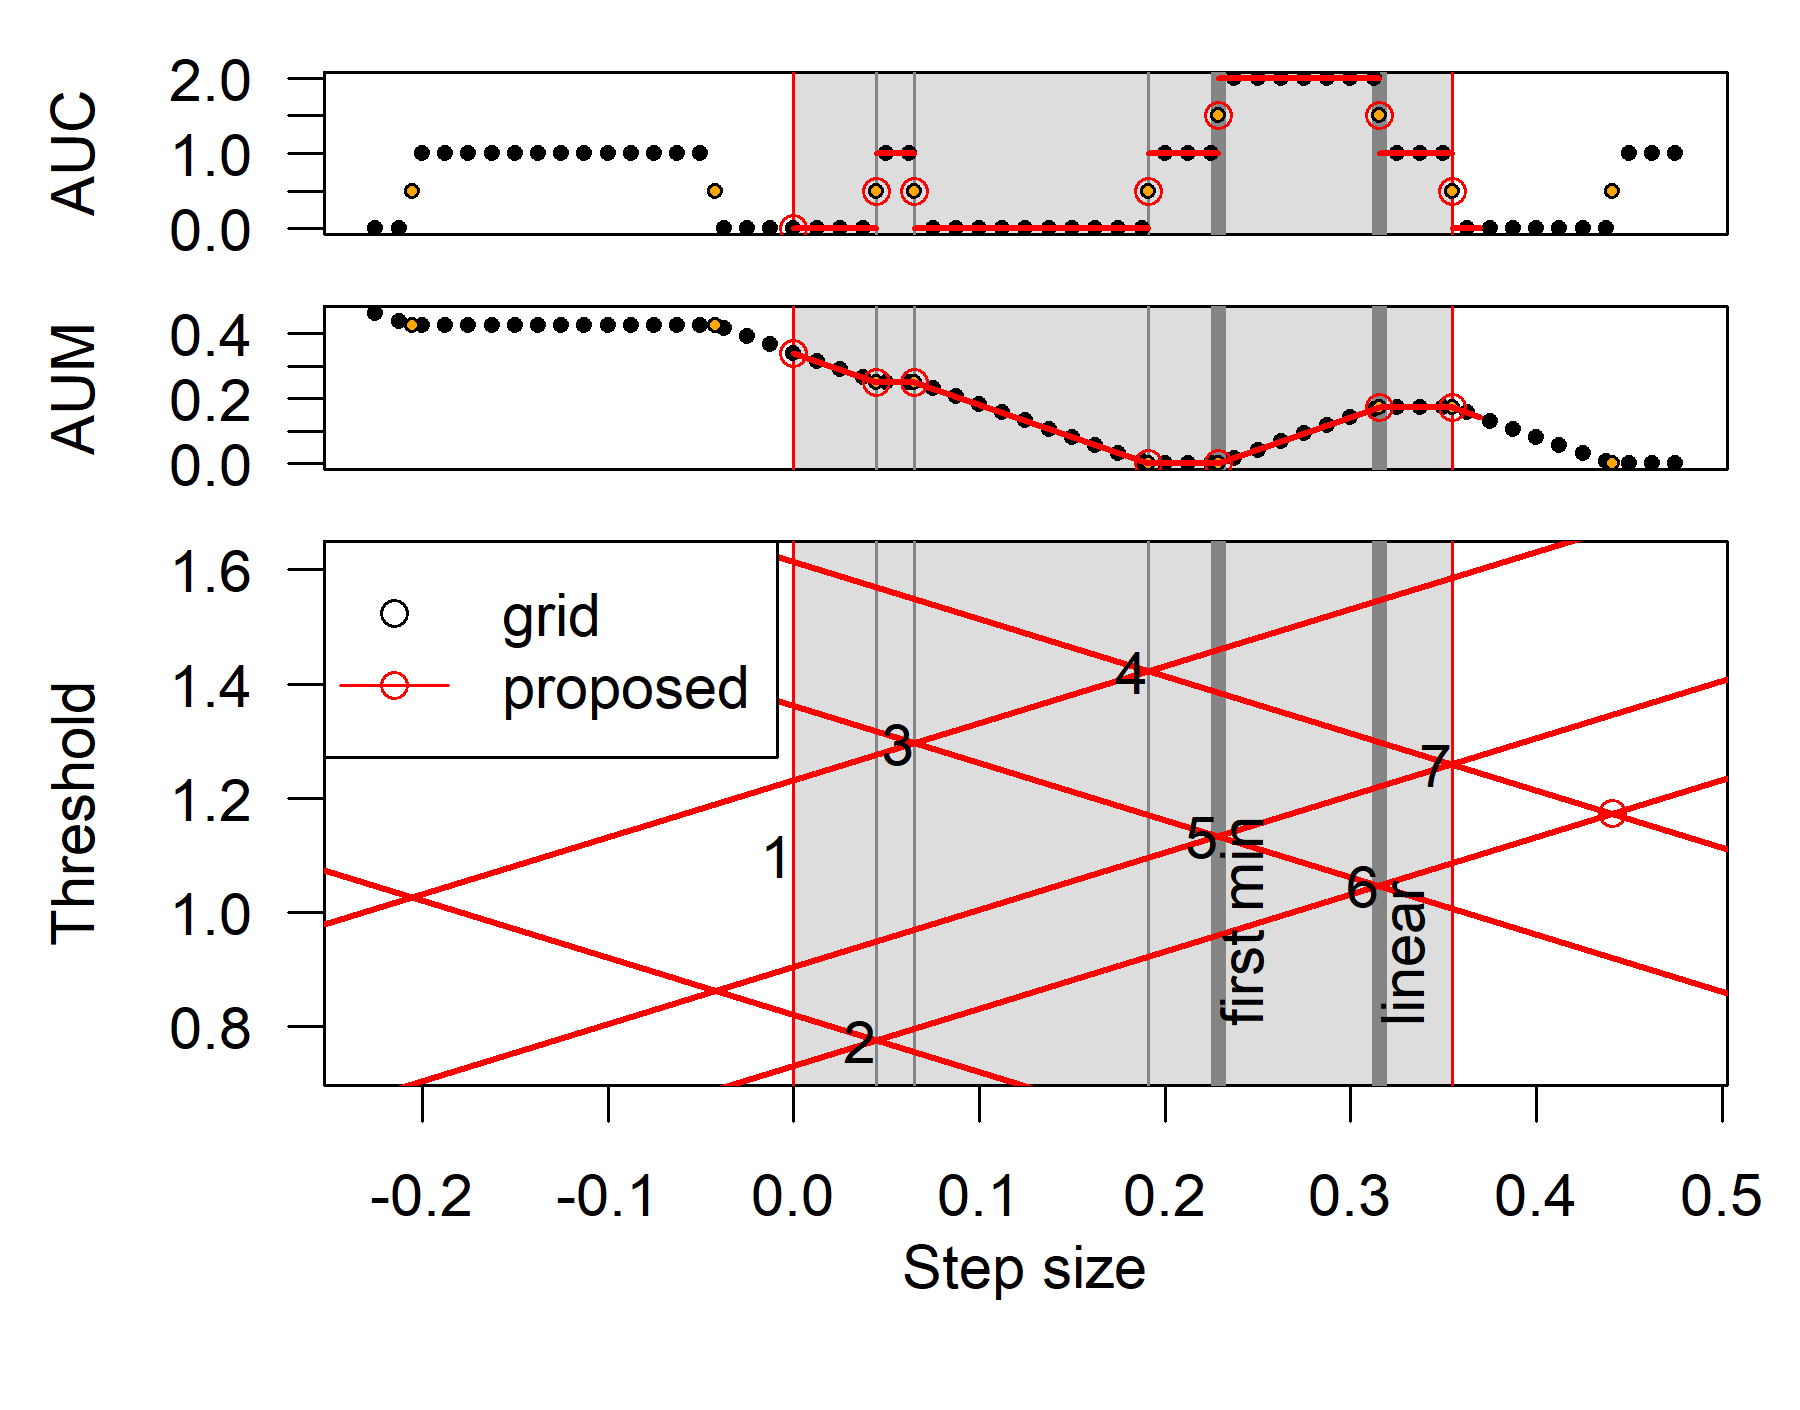
\includegraphics[width=\textwidth]{figure-line-search-example-7}
\end{frame}


\begin{frame}
  \frametitle{AUM/AUC line search, iteration 8}
  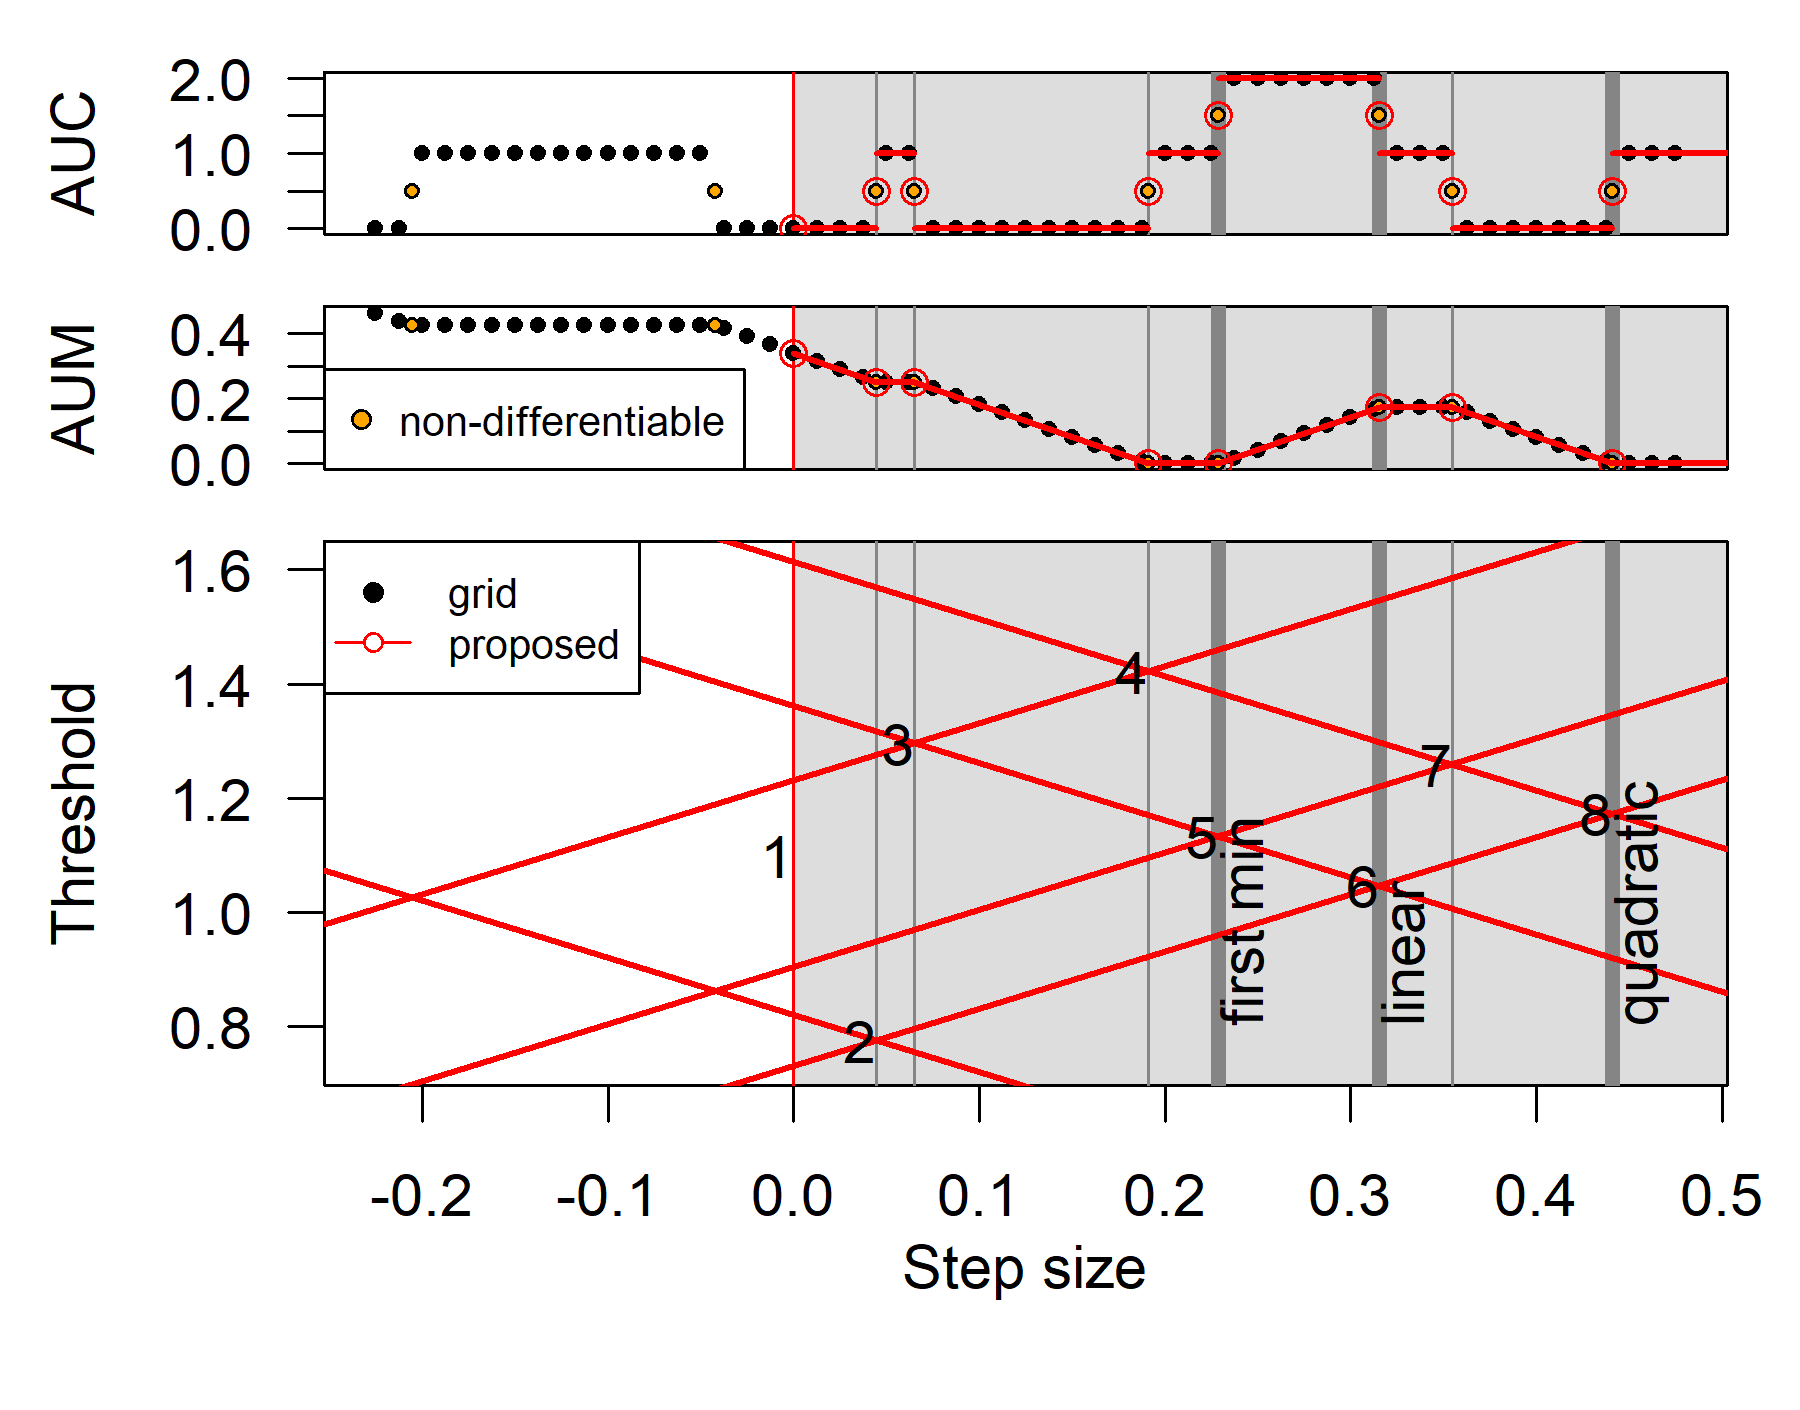
\includegraphics[width=\textwidth]{figure-line-search-example-8}
\end{frame}


\begin{frame}
  \frametitle{Complexity analysis of proposed algorithm}

  For $N$ labeled observations, input $N$ threshold line
  slope/intercept values. Possible next intersection points stored in
  a C++ STL map (red-black tree, sorted by step size), $O(\log N)$
  time insertion, $O(1)$ lookup of next intersection. Worst case $O(N)$
  space.
  %$O([N+I]\log N)$ time for $I$ iterations.
  \begin{description}
  \item[grid: standard grid search.] $O(G N\log N)$ time per step, 
    for $G$ grid points.
  \item[linear(proposed): only first $N$ intersections.]
    $O(N\log N)$ time per step, relatively small step sizes chosen,
    relatively large number of steps overall in gradient descent.
  \item[quadratic(proposed): all $O(N^2)$ intersections.]
    $O(N^2\log N)$ time per step, large step sizes, small number of
    steps.
  \item[first min(proposed): keep iterating until first AUM increase.]
    Same as quadratic in worst case, but may be faster on average (it
    was faster than both quadratic and linear for the example on the
    previous slide).
  \end{description}
\end{frame}

\section{Empirical results: increased speed and comparable accuracy using proposed complete line search} 

\begin{frame}
  \frametitle{AUM gradient descent results in increased train AUC for
    a real changepoint problem}
 
Hillman, Hocking, \emph{Journal of Machine Learning Research} (2023).

\includegraphics[height=3.7cm]{figure-aum-optimized-iterations.png}
\includegraphics[height=3.7cm]{figure-aum-train-both.png}

\begin{itemize}
\item Left/middle: changepoint problem initialized to prediction vector with
  min label errors, gradient descent on prediction vector.
\item Right: linear model initialized by minimizing regularized convex
  loss (surrogate for label error, Hocking \emph{et al.} ICML 2013),
  gradient descent on weight vector.
\end{itemize}

\end{frame}

\begin{frame}
  \frametitle{Proposed search consistently faster than grid search}

  Analyzed supervised genomic change-point detection data set
  H3K4me3\_TDH\_immune ($N=1073$ to 1248)
%     > subtrain.sizes[data.name=="H3K4me3_TDH_immune"]
%             data.name      cv.type test.fold n.subtrain.diffs
% 1: H3K4me3_TDH_immune equal_labels         1             1248
% 2: H3K4me3_TDH_immune equal_labels         2             1200
% 3: H3K4me3_TDH_immune equal_labels         3             1197
% 4: H3K4me3_TDH_immune equal_labels         4             1073
  from UCI Machine Learning Repository,
  {\scriptsize \url{https://archive.ics.uci.edu/ml/datasets/chipseq},}
  Train/test splits defined via 4-fold CV, linear model initialized by
  minimizing regularized convex loss (surrogate for label error,
  Hocking \emph{et al.} ICML 2013), keep doing AUM rate gradient
  descent steps (with line search) until subtrain loss stops decreasing.

  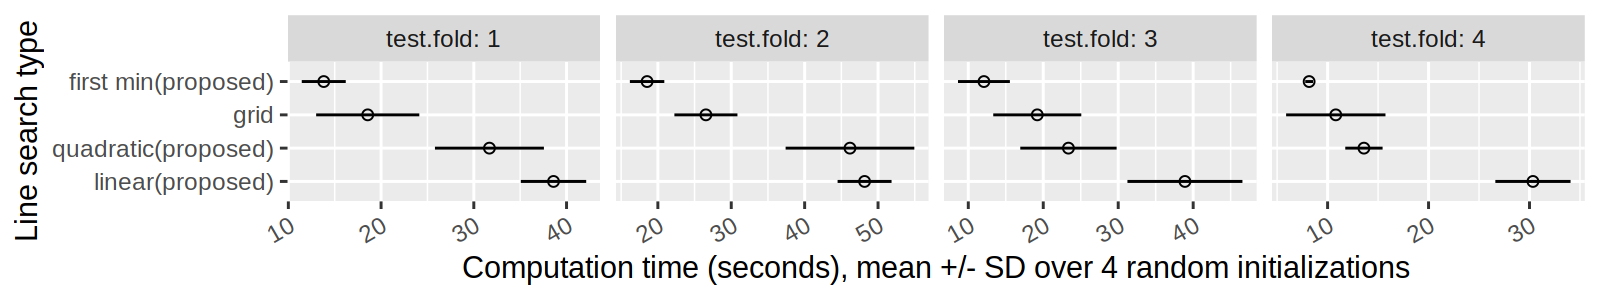
\includegraphics[width=\textwidth]{figure-line-search-complexity-compare-H3K4me3_TDH_immune-equal_labels-rate-IntervalRegressionCV-seconds}

  \begin{description}
  \item[first min(proposed):] keep iterating until first AUM
    increase.
  \item[grid:] search over step
    size$\in\{10^{-9},10^{-8},\dots,10^1,10^0\}$.
  \item[quadratic(proposed):] all line search iterations.
  \item[linear(proposed):] only first $N$ line search iterations.
  \end{description}
\end{frame}

\begin{frame}
  \frametitle{Proposed search has similar accuracy as grid search}

  Analyzed supervised genomic change-point detection data set
  H3K4me3\_TDH\_immune ($N=1073$ to 1248)
%     > subtrain.sizes[data.name=="H3K4me3_TDH_immune"]
%             data.name      cv.type test.fold n.subtrain.diffs
% 1: H3K4me3_TDH_immune equal_labels         1             1248
% 2: H3K4me3_TDH_immune equal_labels         2             1200
% 3: H3K4me3_TDH_immune equal_labels         3             1197
% 4: H3K4me3_TDH_immune equal_labels         4             1073
  from UCI Machine Learning Repository,
  {\scriptsize \url{https://archive.ics.uci.edu/ml/datasets/chipseq},}
  Train/test splits defined via 4-fold CV, linear model initialized by
  minimizing regularized convex loss (surrogate for label error,
  Hocking \emph{et al.} ICML 2013), keep doing AUM rate gradient
  descent steps (with line search) until subtrain loss stops decreasing.

  
\includegraphics[width=\textwidth]{figure-line-search-complexity-compare-H3K4me3_TDH_immune-equal_labels-rate-IntervalRegressionCV-initial}

  \begin{description}
  \item[first min(proposed):] keep iterating until first AUM
    increase.
  \item[grid:] search over step
    size$\in\{10^{-9},10^{-8},\dots,10^1,10^0\}$.
  \item[quadratic(proposed):] all line search iterations.
  \item[linear(proposed):] only first $N$ line search iterations.
  \end{description}
\end{frame}


\section{Discussion and Conclusions}

\begin{frame}
  \frametitle{Discussion and Conclusions}
  \begin{itemize}
  \item Area Under the ROC Curve (AUC) is used to evaluate binary
    classification and changepoint detection algorithms.
  % \item In changepoint detection there can be loops in ROC curves, so
  %   maximizing AUC greater than 1 is not be desirable.
  % \item In changepoint detection, maximizing Area Under ROC curve is
  %   non-trivial even for the train set with unconstrained
  %   predictions.
  \item Hocking, Hillman, \emph{Journal of Machine Learning Research}
    (2023), proposed AUM=Area Under Min(FP,FN), a new
    differentiable surrogate loss for AUC optimization.
  \item In this talk we proposed new gradient descent algorithms with
    efficient complete line search, for optimizing AUM/AUC.
  \item Empirical results provide evidence that proposed complete line
    search is consistently faster than grid search, and has 
    comparable accuracy (in terms of max validation AUC).
  \item Implementations available in R/C++ and python:
    {\scriptsize
    \url{https://cloud.r-project.org/web/packages/aum/} (R/C++ line search)
    \url{https://tdhock.github.io/blog/2022/aum-learning/} (pytorch AUM loss)
    }
  \item Future work: non-linear learning algorithms that use AUM
    minimization as a surrogate for AUC maximization.
  \end{itemize}
\end{frame}

\begin{frame}
  \frametitle{Thanks to co-author Jadon Fowler! (second from left)}

  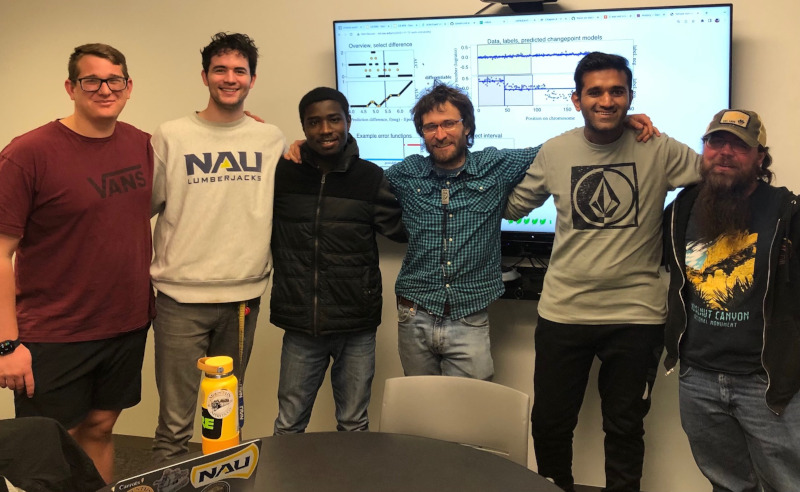
\includegraphics[height=3in]{2023-02-02-group-meeting}

  Contact: toby.hocking@nau.edu

\end{frame} 

\end{document}
